
\section{Ответы на вопросы.}

% Все данные в lisp представляются в форме символьных выражений S-выражений.

% cons == construct (строить) (Городняя: consolidation (укрепление))
% СAR == Contents of Address Register
% CDR == Contents of Decrement Register 

% eval - выполняет двойное вычисление своего аргумента.

% Единая форма записи программы и данных.

% Лисп-программа представляет собой последовательность атомов или списков, 
% которые можно вычислить и получить значение.

% Вместо общепринятой в математике записи обращений к функциям
% вида f(x,y) в Лиспе используется нотация, при которой имя функции
% стоит не перед аргументными скобками, а внутри них, вместе с
% аргументами, которые разделяются уже не запятыми, а пробелами:
% (f x y). Именно за счёт этого достигается синтаксическое единообразие
% программы и данных.

% \begin{lstlisting}
% x => (GAMMA (15))

% (eval (cons (quote car) (quote (x)))) => GAMMA
% 		|---------(car x)---------|

% \end{lstlisting}

\textbf{1. Элементы языка.}

Элементами языка являются атомы и точечные пары.

\textbf{Атомы} представляю из себя:
\begin{enumerate}
	\item Символы - синтаксически представляется как набор букв и цифр, начинающийся с буквы.
	\item Специальные символы - \{T, Nil\}.
	\item Самоопределимые атомы - натуральные, дробные и вещественные числа, а также строки, заключенные в двойные апострофы. 
	% Их значение переопределить нельзя.
\end{enumerate}

Атомы обычно выглядит как последовательность букв или цифр.

Примеры атомов:
\begin{lstlisting}
	B
	CAT
	Я123Атом
	ВотЭтоТожеАтом
	123
	T
	Nil
	2/3
	"abc"
\end{lstlisting}

\textbf{Точечная пара} - (A . B). Строится с помощью бинарных узлов.   

\begin{lstlisting}
	Точечная пара ::= (<атом>.<атом>) |
					  (<атом>.<точечная пара>) |
					  (<точечная пара>.<атом>) |
					  (<точечная пара>.<точечная пара>)	
\end{lstlisting}

Пример точечной пары:
\begin{lstlisting}
(A . (B . (C . (D . Nil))))
\end{lstlisting}
Облегченная форма записи:
\begin{lstlisting}
(A B C D)
\end{lstlisting}

\begin{figure}[ht!]
	\centering{
		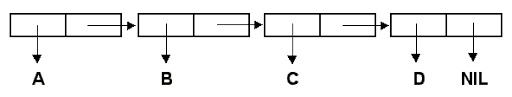
\includegraphics[width=0.9\textwidth]{img/img1}
		\caption{Представление в памяти (A B C D).} }
\end{figure}

\textbf{Представление в памяти:}

\begin{enumerate}
	\item \textbf{(A . B)}
	\begin{figure}[ht!]
		\centering{
			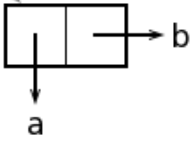
\includegraphics[width=0.2\textwidth]{img/img3}
			\caption{Представление в памяти (A . B).} }
	\end{figure}
	\item \textbf{(A B)} - экономия памяти, но проблема при рекурсивной обработке (т.к. не сможем идентифицировать конец, как Nil)
	\begin{figure}[ht!]
		\centering{
			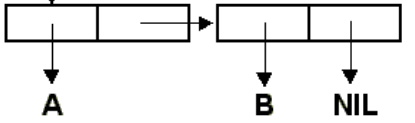
\includegraphics[width=0.5\textwidth]{img/img2}
			\caption{Представление в памяти (A B).} }
	\end{figure}
\end{enumerate}

\begin{lstlisting}
	S-выражение ::= <атом> | <точечная пара>
\end{lstlisting}

Список является частым случаем S-выражения.

S-выражение представлено 

\begin{figure}[ht!]
	\centering{
		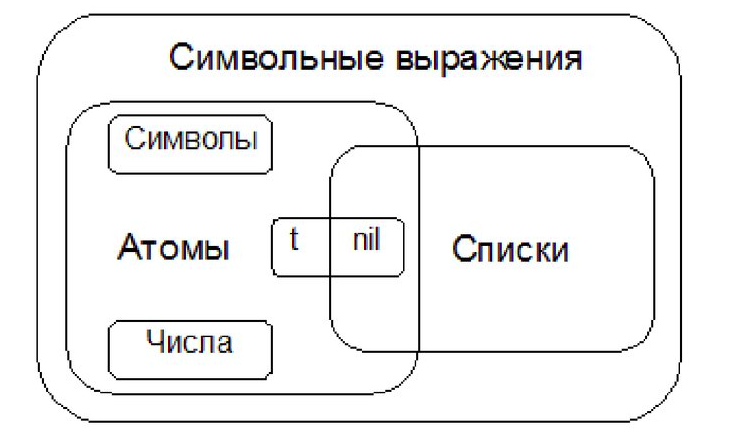
\includegraphics[width=0.5\textwidth]{img/img4}
		\caption{S-выражение} }
\end{figure}

\textbf{Список} - динамическая структура данных, которая может быть
пустой или непустой. Если она не пустая, то состоит из двух элементов:

1. Головы - любая структура.

2. Хвоста - список.

Список представляет из себя заключенную в скобки
последовательность из атомов, разделенных пробелами, или списков.
Любой список является программой - его нужно вычислять.

Примеры списков:
\begin{lstlisting}
	(A B C)
	(1 2 3)
	((A B) (C D))
\end{lstlisting}

\textbf{2. Синтаксис.}

Lisp является регистронезависимым языком. 

Универсальным разделителем, между атомами, является пробел. В начальных версиях была предложена запятая, но она не прижилась.

Наличие скобок является признаком структуры - списка или точечной пары.
% Ограничитель - круглые скобки.

\textbf{Специальные символы:}
\begin{enumerate}
	\item \textbf{T} - Константа. обозначает логическое значение "истина". Истинным значением является все, что отличное от Nil.
	\item \textbf{Nil} - "ложь". Также обозначает пустой список. Записи nil и () эквивалентны. Являются синтаксисом пустого списка
\end{enumerate}

Любая структура заключается в круглые скобки.

(A . B) - точечная пара.

(A) - список из одного элемента.

() или Nil - пустой список.

Одноуровневый список:
\begin{lstlisting}
	(A B C D)
\end{lstlisting}

Структурированный список:
\begin{lstlisting}
	(A (B C) (D E))
\end{lstlisting}

\textbf{3. Как воспринимается символ апостроф}

Символ апостроф - синоним quote.

\textbf{quote} - блокирует вычисление своего аргумента.
В качестве своего значения выдаёт сам аргумент, не вычисляя его.
Перед константами - числами и атомами T, Nil можно не ставить апостроф.
% т.к. значением любой константы является она сама.

Пример использования quote:
\begin{lstlisting}
	(quote (car (A B C))) => (car (A B C))
\end{lstlisting}

% \begin{lstlisting}
% 	(quote (EVAL (ATOM B))) => (EVAL (ATOM B))
% \end{lstlisting}

Вычисление начинается с внешней функции quote, которая возвращает аргумент в неизмененном виде.

\textbf{4. Что такое рекурсия и примеры из lisp}

\textbf{Рекурсия} - это ссылка на описываемый объект в процессе его описания.

% Городняя:
Примером рекурсии в lisp служит S-выражение, которое может быть атомом,
либо заключенная в скобки пара состоящая из S-выражений (разделенных точкой).


